\chapter{Background}
\section{\label{sec:code-representation} Source code representation}
The way we represent source code is very important in code clone detection,
as it affects greatly the algorithms that may be used to detect clones.k
In this section, we will explain the different ways in which source codes
can be represented.
\subsection{\label{ssec:string-representation} String representation}
The most common representation for a program is its string representation. It is
the representation that developer actually uses when editing a program, and
is therefore the easiest to obtain, as it is simply the raw program.
Listing~\ref{lis:add} is a function taking two numbers as input and returning
their sum.
\begin{lstlisting}[caption=\lstinline{add} function,label=lis:add]
int add(int a, int b) {
  return a + b;
}
\end{lstlisting}
The string representation of the above program would simply be
\begin{lstlisting}
"int add(int a, int b) {\nreturn a + b;\n}"
\end{lstlisting}
\subsection{\label{ssec:token-representation}Token representation}
While the string representation is an array of characters, the token
representation is an array of strings where each string in the array is a token
of the program. It is typically the representation that a lexer would return
while processing the source program. The above program would have the following
token representation.
\begin{lstlisting}
["int", "add", "(", "int", "a", ",", "int", "b",
 ")", "{", "return", "a", "+", "b", ";", "}"]
\end{lstlisting}
Token representation may, or may not keep whitespaces and other formatting
characters, but except for programming languages where whitespaces are significant,
such as Python, they are usually not included in the output.
\subsection{\label{ssec:tree-representation}Tree representation}
There are two main tree representations for programs: concrete syntax trees and
abstract syntax trees. We will describe the two different type of trees and
there differences.
\subsubsection{Concrete Syntax Trees}
Concrete syntax trees are concrete in the sense that they keep all the syntactic
tokens of the program, such as commas, semi-colons or parentheses. It therefore
contains exactly the same tokens as the token representation, but the tokens
are organized as a tree, where the root is usually the entry of the program,
the nodes are usually statements or expressions and the leaves are identifiers
or literals. Figure~\ref{fig:add-cst} shows how Listing~\ref{lis:add} would be
represented as a concrete syntax tree.
\begin{figure}[tb]
  \begin{center}
    \includedot[height=5cm]{./diagrams/add-cst.dot}
    \caption{\label{fig:add-cst}Concrete Syntax Tree of \lstinline{add} function}
  \end{center}
\end{figure}
\subsubsection{Abstract Syntax Trees}
Abstract Syntax Trees (AST) are also a tree representation of the source code,
but as opposed to the concrete syntax tree, they do not preserve the host
language syntax, such as parentheses, and instead express these using the
structure of the tree.
AST are typically the what a parser returns when processing the source code, and
are one of the most common representation for various tasks on programs,
including clone detection.
Figure~\ref{fig:add-ast} shows the AST for Listing~\ref{lis:add}.
\begin{figure}[tb]
  \begin{center}
    \includedot[height=5cm]{./diagrams/add-ast.dot}
    \caption{\label{fig:add-ast}Abstract Syntax Tree of \lstinline{add} function}
  \end{center}
\end{figure}
\section{Code clone fundamentals}
In this section, we will first describe the different types of code clones
that appear in the literature, and that we will be using in this thesis.
We will then view the different approaches to code clone detection that can be
found in the literature.
\subsection{Types of code clones}
It is important to define what is implied when two code fragments are
defined as clones. In the literature, code clones are usually
classified into four different types~\cite{Roy07asurvey}, from Type I to Type IV,
where Type I is the ``strongest'', meaning here that the two code fragments are
the most similar, while Type IV is the ``weakest'' --- the two code fragments
share less in common. We will now give a more precise definition of each code
clone type.
\subsubsection{Type I Clones}
Type I code clones types are clones where the code fragment are the same,
except for some variations that do not affect the logic, such as differences
in whitespaces or comments. In the literature, Type I clones are sometimes also
referred to as exact clones.
For example, let us consider the following code fragment.
\begin{lstlisting}[caption=Fibonacci function,label=lis:fibo]
int fibo(int n) {
  if (n <= 1) {
    return n;
  }
  return fibo(n - 1) + fibo(n - 2);
}
\end{lstlisting}

The following code fragment is considered to be a Type I clone.
\begin{lstlisting}
int fibo(int n) {
  if (n <= 1) { return n; } // base case of recursion
  return fibo(n-1)+
         fibo(n-2);
}
\end{lstlisting}

Although, as with the above example, line-by-line comparisons may not always
yield correct results for Type I clones, it is worth noting than if the two
fragments are pre-processed with a lexer, a simple token comparison should
normally be enough to detect this type of clones.
\subsubsection{Type II Clones}
Type II clones include the changes that can be involved in Type I clones, such
as layout and comments, but also include other changes, such as changes in
user-defined identifiers --- variable or function names. For example, the
following snippet would be a Type II clone for Listing~\ref{lis:fibo}:
\begin{lstlisting}
int fib(int x) {
  if (x <= 1) { return x; }
  return fib(x - 1) + fib(x - 2);
}
\end{lstlisting}
The function and parameter names, as well as the layout are different, but the
logic is exactly the same.
\subsubsection{Type III Clones}
Type III clones can have all the changes from type I and type II clones, but
may also have statement insertions, deletions or replacements.
Although Type III clones are usually copied from the same source code,
there is no agreement on a threshold on the number of changes to consider or not
two code fragments as type III clones. Some researchers therefore classify
type III code clones in categories such as very strong type III or weakly type
III~\cite{Sajnani:2016:SSC:2884781.2884877}.
Here is an example type III clone for Listing~\ref{lis:fibo}.
%
\begin{lstlisting}
int fib(int x) {
  int a = x;
  if (a <= 1) {
    return a;
  }
  return fib(a - 1) + fib(a - 2);
}
\end{lstlisting}

In the above code fragment, the code is completely copied from
Listing~\ref{lis:fibo}, except for a change in the identifier names, but the
second line has been inserted, making this code fragment a type III clone.
\subsubsection{Type IV Clones}
Type IV clones, also referred to as functional code clones, are two code
fragments implementing the same functionality with different approaches.
Unlike type I to III clones, type IV clones are usually not a result of
code copying, but rather of two programmers implementing the same functionality.
For example, as opposed to the recursive implementation of Fibonacci in
Listing~\ref{lis:fibo}, the following iterative implementation could be defined
to be a type IV clone.
\begin{lstlisting}[caption=Iterative Fibonacci,label=lis:iter-fibo]
int fib(int n) {
  int a = 0, b = 1;
  for (int i = 0; i < n; i++) {
    int tmp = a + b;
    a = b;
    b = tmp;
  }
  return a;
}
\end{lstlisting}
The two code fragments will return the same result for any $n \geq 0$ and are
therefore functional clones. Although the implemented functionality
is the same, there are no other common point in the implementations.
Furthermore, Listing~\ref{lis:fibo} and Listing~\ref{lis:iter-fibo} clearly
have different time complexities, but to the best of our knowledge, there
are no established convention to whether this kind of complexity changes
should be taken into account when deciding if two code fragments are, or not,
type IV code clones. In this thesis, we will therefore assume that as long
as two code fragments implement same functionality, they are type IV clones.
\subsection{Approaches to clone detection}
There exist various methods to clone detection, which take advantage of the
different source code representations described in
section~\ref{sec:code-representation}. We will present the major
approaches found in the literature.
\subsubsection{Text-based detection}
Text-based clone detection are based on the string representation of the program
source code described in~\ref{ssec:string-representation}.
While some text-based techniques use the source code almost as is and perform
either line-by-line or global string comparisons to find clones, some techniques
do apply some preprocessing steps \cite{Baker92aprogram}, such as removing white
spaces, before actually passing the source code to a string matching algorithm.
\subsubsection{Token-based detection}
Token-based detection techniques use the token representation of the program
described in~\ref{ssec:token-representation}. Token-based approach are usually
more robust to formatting and layout changes compared to text-based approaches.
Some token-based clone detection tools, such as CCFinder
\cite{Kamiya:2002:CMT:636188.636191} first normalize the tokens and replace all
application specific tokens such as user-defined identifiers. On the other hand,
other tools such as SourcererCC \cite{Sajnani:2016:SSC:2884781.2884877} keep
this information and use it to detect if multiple code fragments are clones or
not.
\subsubsection{Tree-based detection}
Tree-based techniques make use of the AST representation of the program
described in \ref{ssec:tree-representation}. These techniques first use a parser
to generate the AST of a program, then the ASTs are searched for similar
sub-trees and similar sub-trees are marked as clones. Searching for similar
sub-trees using normal tree comparisons algorithms takes at least
$\mathcal{O}\left(n^3\right)$ \cite{Baxter:1998:CDU:850947.853341}, where $n$ is
the number of nodes. Industrial software can have millions of line of codes, and
therefore $n$ could be in the order of 10 million. To avoid this issue, many
tree-based clone detection techniques \cite{Baxter:1998:CDU:850947.853341,
  Jiang:2007:DSA:1248820.1248843} use hash functions on sub-tress to find clones
more efficiently. The idea is to assign each sub-tree a hash-value, and use this
value, usually with bucketing techniques, to quickly search for code clones.
\section{Machine learning fundamentals}
In this section, we will present the basics of machine learning that will be
needed in order to understand our approach. We will first give a general
overview of the learning process of neural networks, then we will describe
the two models we are using as a base to our work in this thesis.
The first model will present is the skipgram model, which is typically used in
natural language processing (NLP) to assign a vector representation to a word.
Next, we will give an overview of recurrent neural networks (RNN), and in
particular long-short term memory (LSTM) networks, which are extensively used in
NLP to assign a vector representation to a sentence.
\subsection{Neural networks}
In this subsection, we will show how are neural network composed, and what is
the normal process to train them. Although most of what we explain here apply to
most machine learning algorithms, we will focus on feed-forward neural networks.
\subsubsection{Computations of a neural network}
A neural network \cite{Rojas:1996:NNS:235222} is usually composed of an input
layer, which is where the input data is fed, one or more hidden layers, and an
output layer, which represents the value outputted by the neural network.
Each layer in the network is composed by units, also sometimes referred to as
neurons, which are the computing elements of the network. Each unit is usually
composed of two different parts: a first function $f$, which reduces a vector
into a single scalar value, and a function $g$, called ``activation function''
which transforms the result of $f$ and produces the unit output. This function
is generally non-linear, otherwise the model ends up to be composed of only
linear function and becomes as well a linear function.
A unit of a neural network is illustrated in figure \ref{fig:neuron}.
\begin{figure}[tb]
  \centering% adapted from https://tex.stackexchange.com/questions/365519/draw-single-neural-unit-using-tizk
\begin{tikzpicture}[node distance = 4mm and 12mm,
                    start chain = going below,
                    arro/.style = {-Latex},
                    bloque/.style = {inner sep=1pt, align=right, on chain}]

  \foreach \i [count=\j] in {1, 2, 3}
    \node[bloque] (in-\j) {$x_{\i}$};
  \node (out) [circle, draw, minimum size=6mm, right=of $(in-2)!0!(in-3)$] {};

  \foreach \i in {1,...,3}
    \draw[arro] (in-\i) -- (out);
  \coordinate[right=of out] (output);
  \draw[arro] (out) -- (output) node[right] {$g\left(f(x_1,\cdots,x_n)\right)$};
\end{tikzpicture}

  \caption{\label{fig:neuron}Unit of a neural network}
\end{figure}
Each layer is connected to the next one by using the output of each unit of the
previous layer as an input for each unit of the next layer. This connection is
illustrated in figure \ref{fig:neural-net}.
\begin{figure}[tb]
  \centering% taken from https://tex.stackexchange.com/questions/132444/diagram-of-an-artificial-neural-network
\begin{tikzpicture}[
plain/.style={
  draw=none,
  fill=none,
  },
net/.style={
  matrix of nodes,
  nodes={
    draw,
    circle,
    inner sep=10pt
    },
  nodes in empty cells,
  column sep=2cm,
  row sep=-9pt
  },
>=latex
]
\matrix[net] (mat)
{
|[plain]| \parbox{1.3cm}{\centering Input\\layer} & |[plain]| \parbox{1.3cm}{\centering Hidden\\layer} & |[plain]| \parbox{1.3cm}{\centering Output\\layer} \\
& |[plain]| \\
|[plain]| & \\
& |[plain]| \\
  |[plain]| & |[plain]| \\
& & \\
  |[plain]| & |[plain]| \\
& |[plain]| \\
  |[plain]| & \\
& |[plain]| \\    };
\foreach \ai [count=\mi ]in {2,4,...,10}
  \draw[<-] (mat-\ai-1) -- node[above] {$x_\mi$} +(-2cm,0);
\foreach \ai in {2,4,...,10}
{\foreach \aii in {3,6,9}
  \draw[->] (mat-\ai-1) -- (mat-\aii-2);
}
\foreach \ai in {3,6,9}
  \draw[->] (mat-\ai-2) -- (mat-6-3);
\draw[->] (mat-6-3) -- node[above] {Ouput} +(2cm,0);
\end{tikzpicture}

  \caption{\label{fig:neural-net}Neural network}
\end{figure}

The function $f$ is a matrix multiplication where all the weights of this matrix
are parameters of the neural network model. Matrix weights are shared by all the
units in a layer. In figure \ref{fig:neural-net}, given $W^{(1)} \in
\mathbb{R}^{5\times 3}$ is the matrix weights of the hidden layer, $W_{mn}$ is
the value at row $m$ and column $n$ in this matrix, $g_1$ is the activation
function of the hidden layer, and $a_1, a_2$ and $a_3$ the output of each unit
in the layer, we will have the following.
\begin{align*}
  a_1 &= g\left( W_{11}^{(1)}x_1 + \cdots + W_{51}^{(1)}x_5 \right)\\
  a_2 &= g\left( W_{12}^{(1)}x_1 + \cdots + W_{52}^{(1)}x_5 \right)\\
  a_3 &= g\left(W_{13}^{(1)}x_1 + \cdots + W_{53}^{(1)}x_5 \right)
\end{align*}
In practice, given $x = (x_1, \cdots, x_5)$ and $a = (a_1, a_2, a_3)$, the above
is usually computed as follow, with a single matrix multiplication and a
vectorized implementation of the function $g$.

\[ a = g\left(  x W^{(1)}  \right) \]

Finally, given $W^{(2)} \in \mathbb{R}^{3\times 1}$ the weights of the output
layer and $g_2$ the activation of the output layer, the output $\hat{y}$ of the neural
network will be computed as follow.

\begin{equation}
  \hat{y} = g_2\left( g_1\left( x W^{(1)} \right) W^{(2)} \right)
\end{equation}
\subsubsection{Training of a neural network}
Training a neural network is searching for the optimal weights to approximate
the function the neural network should learn. In the above example, this process
consists in searching values for $W^{(1)}$ and $W^{(2)}$.
The ``optimal'' weights of a neural network are defined with respect to a loss
function representing how far the neural network output is from the expected
correct answer, which is chosen depending on the task. Some common loss
functions include mean squared error (MSE) \ref{eq:mse} or cross-entropy
error (CEE) \ref{eq:cee}. Given a set of outputs $\hat{Y} = \{ \hat{y_1}, \cdots,
\hat{y_n} \}$ and their respective expected values $Y = \{ y_1, \cdots,
y_n \}$, the errors are defined as follow.

\begin{align}
  \label{eq:mse}MSE(\hat{Y}, Y) &= \frac{1}{n}\sum_{i=1}^{n} \left( y_i - \hat{y_i} \right)^2\\
  \label{eq:cee}CEE(\hat{Y}, Y) &= \frac{1}{n}\sum_{i=1}^{n}
                                  y_i\log\hat{y_i} + (1 - y_i)\log(1 - \hat{y_i})
\end{align}
Mean squared error is typically used when there is an order relation between the
possible outputs while cross-entropy error is mostly used for classification
tasks where the output can either be correct or incorrect.

The most common way to update the weights of the neural network is called the
back propagation algorithm, and consists in computing the derivatives of the
loss function with respect to the weights of the model using the derivative
chain rule, and to use these to update the weights with optimization methods
such as the gradient descent. For example, given a loss function $L(W)$, to
update $W^{(2)}$ in the above network, we would compute the error derivative
$\partial L(W)/\partial W^{(2)}$, multiply the result with a learning
rate $\alpha$, which is a hyper parameter of the model, and subtract the result
from the current value of $W^{(2)}$. This process is usually repeated until the
error converges.
\subsection{Skipgram model}
As mentioned above, skipgram is used to assign a vector in $\mathbb{R}^d$, known
as a word embedding, to a word, where $d$ is the number of dimensions wanted for
each word vector. This algorithm has first been presented in 2013 by Mikolov \&
al. \cite{DBLP:journals/corr/MikolovSCCD13} and is now used in many natural
language processing tasks as one of the word2vec algorithms.

To understand the motivations behind this algorithm, and other algorithms used
to learn word embeddings, we must first understand how words used to be
represented in natural language processing tasks. The most common approach was
to use a finite vocabulary of size $|V|$, and to assign an identifier to each
word in this vocabulary. For example, the word ``network'' could have the id
$123$, and would be represented as a vector in $\{0,1\}^{|V|}$ where only index
$123$ of the vector would be $1$ and all the other indexes would be $0$. This
approach has two disadvantages: each word is represented by a very large and
sparse vector, and the representation of each word do not have any semantic
properties, so ``network'' and ``networks'' vector representations would not be
any closer than ``network'' and any other word representation.

The motivation behind skipgram is to address this issue by encoding each word
as a vector in $\mathbb{R}^d$ where $d$ is not dependent of $|V|$, in such a way
that each word embedding has some semantic so that, for example, similar words
have a smaller distance in $\mathbb{R}^d$ than unrelated words.

We will now describe how the skipgram algorithm actually computes the vector
embeddings for each word. The algorithm works in an unsupervised fashion and
usually uses a large amount of text written in the language of the vocabulary.
For each sentence, a set of training samples composed of a ``context'' word and
a ``target'' word. The context word is a word in the sentence, while the target
word is a word around the context word, which is distant by at most a predefined
window size. For example, if the window size is 2, and we have the following
sentence,
\begin{quotation}
the quick brown fox jumped over the lazy dog
\end{quotation}
the target words for the context word ``fox'' will be ``quick'', ``brown'',
``jumped'' and ``over''. These samples are used to train a neural network with a
single hidden layer. The word embeddings are the hidden layer of the network and
have dimension $\mathbb{R}^{|V|\times d}$. The network is trained by using the context
word index to select a vector from the hidden layer weight and using a
cross-entropy error function so that when the word is a target, the label should
be $1$ and $0$ otherwise. Also this could be done by using a softmax output,
this would require to compute softmax on all the vocabulary, which can be
extremely large. To reduce the computation cost, a common approach is to used
negative sampling. The negative sampling approach only computes the output for
the target word, as well as a predetermined number of noise word --- word
not in the window of the context --- and uses the sum of these errors to train
the model.
\subsection{Recurrent Neural Networks}
While word embeddings work well to represent a single word, and to model the
similarities between words, it is not enough to encode a whole sentence. There
are many approaches to encode a sentence into a vector, and Recurrent Neural
Networks (RNN) is one of them. The main idea of RNNs is to reuse the previous
output as an input, as shown in \ref{fig:rnn}.
\begin{figure}[tb]
  \begin{center}
    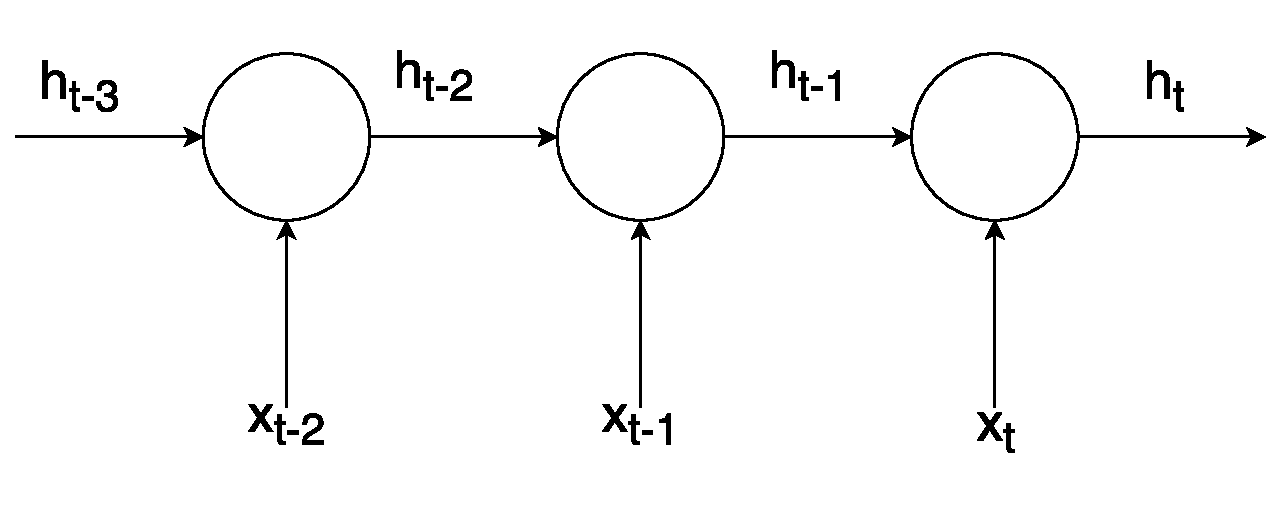
\includegraphics[width=8cm]{./images/rnn.pdf}
    \caption{\label{fig:rnn}Unrolled Recurrent Neural Network}
  \end{center}
\end{figure}
Typically, each $x_t$ is a word in the sentence, encoded either as a
one-hot vector or as a word embedding. In its simplest form, a RNN will compute
its output using equation \ref{eq:rnn}, where $W$, $U$ and $b$ are parameters of
the model. The parameters are shared across all time steps.
\begin{equation}
  h_t = \tanh\left( W x_t + U h_{t - 1} + b \right) \label{eq:rnn}
\end{equation}
Although this models seems promising, it suffers a major issue --- it is very
difficult to capture long-term dependencies because of the vanishing gradients
issue \cite{pascanu2013difficulty}. When computing the gradients to
back-propagate the error through the network, the gradient for $\partial x_t$
with respect to $\partial x_k$, used in the chain rule, can be expanded as
follow.
\begin{equation}
  \frac{\partial x_t}{\partial x_k} = \prod_{t \geq i > k} \frac{\partial x_i}{\partial x_{i-1}}
  \label{eq:rnn-vanishing-gradients}
\end{equation}
The term $\partial x_i/\partial x_{i-1}$ in equation
\ref{eq:rnn-vanishing-gradients} is less then $1$ \cite{pascanu2013difficulty},
which means that the value will converge to $0$, and error will not propagate
all the way through the network, hence the vanishing gradient issue.

To overcome this issue, Long Short-Term Memory (LSTM) networks
\cite{Hochreiter:1997:LSM:1246443.1246450} are often used instead of vanilla RNN
described above. Instead of equation \ref{eq:rnn}, LSTMs use equations
\ref{eq:lstm-1} to \ref{eq:lstm-6} to compute the output value. All $W$, $U$ and
$b$ in the equations are parameters of the model.
\begin{align}
  f_t &= \sigma \left( W^{(f)}x_t + U^{(f)}h_{t - 1} + b^{(f)} \right) \label{eq:lstm-1}\\
  i_t &= \sigma \left( W^{(i)}x_t + U^{(i)}h_{t - 1} + b^{(i)} \right)\\
  u_t &= \tanh \left( W^{(u)}x_t + U^{(u)}h_{t - 1} + b^{(u)} \right)\\
  o_t &= \sigma \left( W^{(o)}x_t + U^{(o)}h_{t - 1} + b^{(o)} \right)\\
  c_t &= i_t \odot u_t + f_t \odot c_{t - 1}\\
  h_t &= o_t \odot \tanh(c_t) \label{eq:lstm-6}
\end{align}
In the above equations, $\sigma$ is the sigmoid function defined by equation
\ref{eq:sigmoid},
\begin{equation}
  \sigma(x) = \frac{1}{1 + e^{-x}} \label{eq:sigmoid}
\end{equation}
and the different values have the following meaning.
\begin{description}
\item[$f_t$] - forget gate - how much of the previous state should be used
\item[$i_t$] - input gate - how much of the input should be used
\item[$u_t$] - update gate - the value of the current input
\item[$o_t$] - output gate - how much of the current result should be outputted
\item[$c_t$] - memory cell - the state of the network
\item[$h_t$] - hidden layer - the output of the LSTM cell
\end{description}
Given $g^n(x_t, h_{t-1}) = W^{(n)}x_t + U^{(n)} h_{t-1} + b^{(n)}$, figure
\ref{fig:lstm-cell} shows how the inputs flow in equations \ref{eq:lstm-1} to
\ref{eq:lstm-6} to generate the outputs of an LSTM cell.
\begin{figure}[tb]
  \begin{center}
    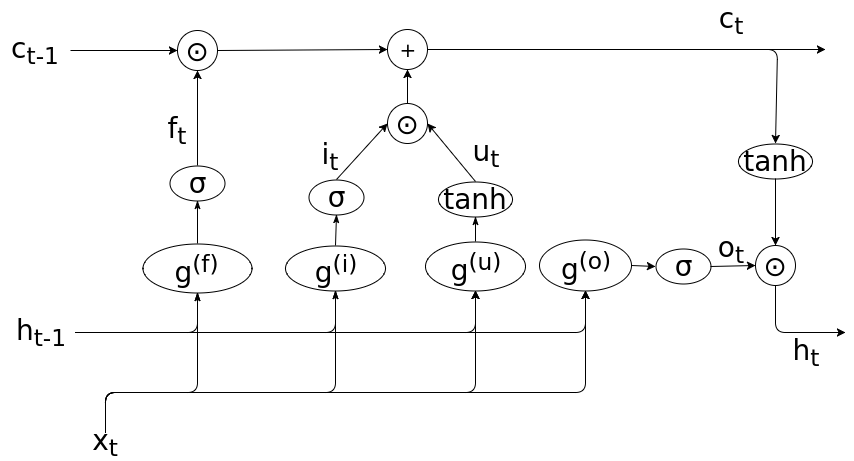
\includegraphics[width=14cm]{./images/lstm-cell.png}
    \caption{\label{fig:lstm-cell}LSTM cell}
  \end{center}
\end{figure}
In an LSTM network, the state is not passed through $h_t$ as with a plain RNN,
but through $c_t$, called the memory cell. Due to the additive nature of $c_t$,
the error will also be propagated in an additive manner when computing the
derivative for $c_t$ \cite{Hochreiter:1997:LSM:1246443.1246450}, avoiding the
vanishing gradient problem encountered when using plain RNNs.
%
\section{Motivating example}
With the proliferation of programming languages, a single project or application
is often written using multiple programming languages. For example, a project
having a native client for the web, Android and iOS will most likely have at
least a part of it written in JavaScript, a part written in Java or Kotlin and
another part written in Swift or Objective C. A common issue with such a project
is having a large amount of logic duplicated for each client. In many cases,
business logic for an application with multiple frontends can be extracted to
the backend to avoid duplication.
